\documentclass{article}
\usepackage[utf8]{inputenc}
\usepackage{amsmath}
\usepackage{graphicx}
\usepackage[top=1.55cm, bottom=2.29cm, left=1.6cm, right=1.47cm]{geometry}

% This is for the fancy title in each page
\usepackage{fancyhdr}
\lhead{}
\chead{}
\rhead{First Session: Combinational Design}
\pagestyle{fancy}

% This is for the karnaugh maps
\usepackage{tikz}
\usetikzlibrary{calc}
\usetikzlibrary{positioning}
\usetikzlibrary{matrix}

\pgfdeclarelayer{background}
\pgfsetlayers{background,main}


\begin{document}

%%%% FRONTPAGE %%%%%%%%%%%%%%%%%%%%%%%%%%%%%%%%%%%%%%%%%%%%%%%%%%%%%%%%%%%
\begin{titlepage}

\begin{center}
%
\includegraphics[width=0.25\textwidth]{./uc3m.jpg}\\[2cm]
\textsc{\LARGE Universidad Carlos III de Madrid}\\[0.5cm]
\textsc{\Large Systems of Perception}\\[4cm]


% Title
{\Huge \bfseries{GECKO\\[1cm] Gesture Recognition}\\[8cm]}


% Author and supervisor
\begin{minipage}{0.55\textwidth}
\begin{flushleft} \large
\emph{Authors:}\\
David Estévez Fernández, 100282441\\
Irene Sanz Nieto, 100282826\\
\end{flushleft}
\end{minipage}
\begin{minipage}{0.4\textwidth}
\begin{flushright} \large
\emph{Teacher:}\\
ABDULLA HUSSEIN ABDULRAHM AL KAFF
\end{flushright}\end{minipage}\vfill

% Bottom of the page
{\large \today}

\end{center}
\end{titlepage}

%
\newpage
%
%%%%%%Table of contents%%%%%%%%%%%%%%%%%%%%%%%%%%%%%%
%%%%%%%%%%%%%%%%%%%%%%%%%%%%%%%%%%%%%%%%%%%%%%%%%%%%%
\tableofcontents
\newpage

%%%%%% Memoria %%%%%%%%%%%%%%%%%%%%%%%%%%%%%%%%%%
%%%%%%%%%%%%%%%%%%%%%%%%%%%%%%%%%%%%%%%%%%%%%%%%%%%%%
\section{Introduction}
In this document a gesture recognition software named GECKO is presented. This software will allow the user to interact with a computer using just hand gestures. 

\subsection{Motivation}

\subsection{First Steps}

\subsection{Final Solution}

\section{User Guide}
This code was developed using the following libraries: 
\begin{itemize}
\item OpenCV (v2.4.6.1).
\item X11 (linux native libraries that allows the control of the windows and mouse). 
\end{itemize}
The software was compiled using CMAKE (minimum version 2.8).
\\[0.5cm]
Therefore, those libraries are needed for the correct functioning of the software. 


\subsection{Compile the software [UBUNTU]}

In order to compile the code, there are various options. Here it will be explained how to compile using qt and terminal. 

To open the software as a Qt project, the only thing needed is to open the main CMakeLists.txt (gecko/CMakeLists.txt) with QtCreator. This will parse the whole project. 
Afterwards, press the "build" icon to build the project. 


The folder structure used is the typical of a CMake project. In order to compile using the terminal follow this steps: 
\begin{enumerate}
 \item Open a terminal in the build directory (gecko/build). 
 \item Enter the command "cmake ..". 
 \item Enter the command "make". 
\end{enumerate}

\subsection{Use the software}
In order to execute the software, press the convinient button of the QtCreator IDE or open a terminal in the bin directory (gecko/bin) and enter the command "./hand.cpp". 

Once the code is compiled and started, a first window will appear with the information about the software. After pressing enter to continue, this menu will pop up: 
\begin{center}
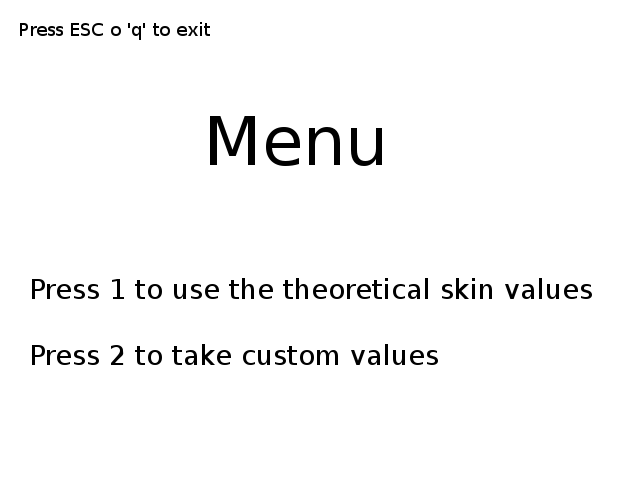
\includegraphics[scale=0.5]{../../img/menu.png} 
\end{center}

The first option will take the theoretical HSV skin values proposed in \textbf{[CITE]}. Afterwards, the application will allow us to adjust those HSV ranges to adecuate them to the room's conditions. 
Once all the adjustments are done, pressing ENTER will start the program. 

The second option will pop up a window with a green square in the middle. Place the hand so that the square is in the middle of your palm and press ENTER. The program will automatically calculate the HSV range of your skin. Afterwards you will be able once more to manually adjust those ranges. Pressing ENTER one last time will start the program. 
\\
\textbf{[EXPLAIN EVERYTHING ABOUT THE GESTURES]}
\section{Software Documentation}
\textbf{[PASTE DOXYGEN OUTPUT]}

\end{document}